\documentclass[12pt,a4paper]{report}

%% ───────────── PACKAGES ─────────────
\usepackage{fontspec}   % for custom fonts (XeLaTeX/LuaLaTeX)
\usepackage{polyglossia} % for multilingual support
\usepackage[hidelinks]{hyperref}
\usepackage{float}
\usepackage{multirow} 
\usepackage{hyperref}
% or
\usepackage{url}
\usepackage{glossaries}
\makeglossaries
\usepackage{booktabs}
\setmainlanguage{english}
\setotherlanguages{arabic,french}
\usepackage{natbib}
\usepackage{float}
\newfontfamily\arabicfont[Script=Arabic]{Arial Unicode MS} % Arabic font (Unicode fallback)
\newcommand{\ar}[1]{\textarabic{#1}} % shortcut for Arabic text
\makeglossaries


\usepackage[margin=2.5cm]{geometry} % ONLY HERE
% Do NOT load geometry again

\usepackage{graphicx}  % for images
\usepackage{booktabs}  % tables
\usepackage{amsmath}   % math
\usepackage{enumitem}  % lists
\usepackage{xcolor}    % colors
\usepackage{tikz}      % diagrams
\usetikzlibrary{positioning, arrows.meta}
\usepackage{geometry}
\geometry{a4paper, top=2.5cm, bottom=2.5cm, left=3cm, right=2.5cm}

\usepackage{setspace}
\onehalfspacing

\setlength{\parskip}{0pt}
\setlength{\parindent}{1.5em}

\usepackage{titlesec}
\titlespacing*{\chapter}{0pt}{-10pt}{20pt}
\titlespacing*{\section}{0pt}{12pt}{6pt}
\titlespacing*{\subsection}{0pt}{10pt}{4pt}

\usepackage{enumitem}
\setlist{noitemsep, topsep=4pt}

\usepackage{caption}
\captionsetup{skip=4pt}

\usepackage{hyperref}  % links (last)


%% ───────────── DOCUMENT ─────────────


\graphicspath{{figures/}}
\usepackage{array}


% ---------- Easy customization ----------
\newcommand{\projecttitlea}{Towards Dialogue Systems for Low-Resource Languages: 
A Case Study of the Tunisian Dialect with Code-Switched Speech Recognition and Language Model Adaptation, from Fine-Tuning to Application Integration}
\newcommand{\academicyear}{2025 -- 2026}
% ---------------------------------------

\setlength{\parskip}{0.35em}
\setlength{\parindent}{0pt}

\begin{document}

% ===== Top header with small logos =====
\begin{center}
  \begin{minipage}[c]{0.12\textwidth}\raggedright
    \IfFileExists{logo1.jpg}{
\includegraphics[width=\linewidth]{logo1.jpg}}{}
  \end{minipage}
  \begin{minipage}[c]{0.68\textwidth}\centering
    \textbf{RÉPUBLIQUE TUNISIENNE}\\
    {\small Ministère de l’Enseignement Supérieur et de la Recherche Scientifique}\\
    Université de Carthage\\
    {\small Institut National des Sciences Appliquées et de Technologie (INSAT)}
  \end{minipage}
  \begin{minipage}[c]{0.16\textwidth}\raggedleft
    \IfFileExists{logo 2.png}{
\includegraphics[width=\linewidth]{logo 2.png}}{}
  \end{minipage}
\end{center}

\vspace{0.3cm}
\vspace{3em}
% ===== Main title area =====

\begin{center}
\Large
\textbf{End of year project}\\[3em]

\centerline{\rule{0.85\textwidth}{0.4pt}}
\vspace{0.6cm}

{\large\bfseries \projecttitlea\\ }

\vspace{0.6cm}
\centerline{\rule{0.85\textwidth}{0.4pt}}
\end{center}

% ===== Prepared by / Company / Supervisor =====
\vspace{1cm}

\begin{center}
\Large
\textbf{Presented by}\\[1.25em]
Smati Syrine \\
Ben Ayed Mohamed Ala \\
Sassi Yasmine \\

\end{center}

\vspace{0.25cm}



\vspace{1cm}

\begin{center}

\vspace{0.25cm}
\textbf{Academic Year:} \academicyear
\end{center}

\tableofcontents
\listoffigures
\listoftables

\newpage
\newpage



\chapter{Introduction}
\label{chap:introduction}

%% =====================================================
\section{Motivation and Context}
%% =====================================================

Tunisian Arabic, locally known as \textbf{Derja}, is the primary spoken language of over
12~million Tunisians. Far from being a simplified form of Modern Standard Arabic~(MSA),
Derja is a linguistically rich variety shaped by centuries of contact with French, Italian,
Turkish, and Berber. As a result, it differs substantially from MSA in phonology,
morphology, vocabulary, and syntax, while also remaining distinct from neighbouring Arabic
dialects such as Moroccan Darija and Egyptian Arabic. Despite its central role in everyday
communication, Tunisian Arabic remains severely underrepresented in natural language
processing~(NLP).

One of the defining challenges of Derja is the absence of a standardized writing system.
In digital communication, speakers alternate freely between Arabic script and Arabizi, a
Latin-based transcription system, while frequently code-switching with French and English.
Although these practices reflect authentic linguistic behaviour, they pose major challenges
for NLP systems that rely on stable and standardized input.

Recent advances in Arabic NLP have largely focused on MSA and a small number of
better-resourced dialects, particularly Egyptian and Levantine Arabic. Tunisian Arabic,
by contrast, suffers from limited corpora, benchmarks, and evaluation resources, leading
to weaker model performance and slower research progress. Addressing this gap requires
simultaneous effort in data collection, model adaptation, and evaluation.

Recent multilingual models make this objective increasingly feasible. Large language models
such as AYA-Expanse~\citep{dang2024ayaexpansecombiningresearch} provide multilingual
representations that can be adapted to low-resource dialects through continued pretraining
and fine-tuning. Similarly, Whisper~\citep{radford2022robustspeechrecognitionlargescale}
has demonstrated strong multilingual speech recognition capabilities across dialectal
Arabic varieties. Together, these models offer a practical foundation for building
end-to-end spoken dialogue systems for Tunisian Arabic.%% =====================================================
\section{Target System}
\label{sec:target}
%% =====================================================

The objective of this work is to design, implement, and evaluate a robust end-to-end spoken
dialogue system for Tunisian Arabic, capable of understanding code-switched speech and
generating linguistically authentic, culturally grounded responses. The system integrates
two primary components — an ASR module and a dialect-adapted large language model~(LLM) —
within a unified pipeline that supports natural interaction in Derja, even when
code-switching with French, English, or Berber is present.

\begin{figure}[H]
    \centering
    \begin{tikzpicture}[
        node distance=2.5cm,
        module/.style={
            rectangle, draw=black, fill=white, thick, rounded corners,
            minimum width=3.5cm, minimum height=1cm, font=\footnotesize,
            text width=3cm, align=center
        },
        arrow/.style={->, thick, >=Stealth}
    ]
        \node[module] (asr) {ASR Module \\ \small Transcribe speech};
        \node[module, right=of asr] (dm) {Dialogue Management \\ \small Intent \& context};
        \node[module, right=of dm] (llm) {LLM Generator \\ \small Tunisian Arabic replies};
        \draw[arrow] (asr) -- (dm);
        \draw[arrow] (dm) -- (llm);
        \node[module, above=1cm of asr, fill=gray!15, draw=black]
            (userin) {User Input \\ \small Tunisian Arabic / code-switched speech};
        \node[module, below=1cm of llm, fill=gray!15, draw=black]
            (userout) {System Output \\ \small Response in Tunisian Arabic};
        \draw[arrow, dashed] (userin) -- (asr);
        \draw[arrow, dashed] (llm) -- (userout);
    \end{tikzpicture}
    \caption{High-level architecture of the target spoken dialogue system.}
    \label{fig:target-system}
\end{figure}

\subsection{System Objectives}

The target system is designed to fulfil the following objectives:

\begin{itemize}
    \item Accurately transcribe spoken Tunisian Arabic, including code-switched utterances,
          into a consistent text representation.
    \item Understand user intent and maintain conversational context using a
          dialect-adapted language model.
    \item Generate responses that are semantically accurate, culturally appropriate, and
          faithful to authentic Tunisian Arabic usage.
    \item Handle the orthographic variability inherent in both Arabic script and Arabizi
          input without performance degradation.
    \item Operate on standard hardware at latency suitable for interactive dialogue,
          targeting a response time of under two seconds per user turn.
\end{itemize}

\subsection{System Architecture}

The system follows a modular, pipeline-based architecture comprising three primary
components:

\begin{enumerate}
    \item \textbf{ASR Module.} Converts code-switched spoken input into Arabic-script
          transcripts, handling both dialect-specific phonetic patterns and cross-lingual
          code-switching phenomena.

    \item \textbf{Dialogue Management Module.} Acts as the bridge between transcription
          and response generation. It interprets ASR output, infers user intent, and
          maintains conversational context across turns.

    \item \textbf{LLM-Based Response Generator.} Produces linguistically authentic
          responses in Tunisian Arabic, drawing on a dialect-adapted language model
          augmented with a cultural knowledge base via retrieval-augmented
          generation~(RAG).

    \item \textbf{Retrieval-Augmented Generation (RAG) Module.} Grounds response
          generation in a curated cultural and linguistic knowledge base specific to
          Tunisian Arabic. At inference time, the module retrieves the most semantically
          relevant passages using dense vector search, which are then supplied as
          additional context to the LLM, reducing hallucination and improving dialectal
          and cultural fidelity.
\end{enumerate}

\subsection{Target Use Cases}

The system is designed to support a range of practical applications, including:

\begin{itemize}
    \item Voice-enabled digital assistants for Tunisian Arabic speakers.
    \item Educational tools for language learning and dialect documentation.
    \item Cultural and tourism information systems requiring local dialect comprehension.
    \item Customer service and social media monitoring in Tunisian Arabic.
\end{itemize}

\subsection{Performance Targets}

The following quantitative targets guide the system design and evaluation:

\begin{itemize}
    \item \textbf{ASR accuracy:} Word Error Rate~(WER) below 35\% on code-switched speech.
    \item \textbf{Dialectal fidelity:} High LLM adherence to Tunisian Arabic usage,
          minimising semantic drift toward MSA.
    \item \textbf{Robustness:} Reliable processing of both Arabic-script and Arabizi
          input, as well as mixed-language utterances.
    \item \textbf{Latency:} End-to-end response time under two seconds per dialogue turn
          under standard hardware conditions.
\end{itemize}

%% =====================================================
\section{Research Challenges}
\label{sec:challenges}
%% =====================================================

Developing a spoken dialogue system for Tunisian Arabic requires addressing a constellation
of interrelated challenges that span both ASR and language modelling. These challenges arise
from the linguistic properties of Derja itself, the scarcity of dedicated resources, and the
limitations of existing multilingual systems when applied to this dialect.

\subsection{Shared Challenges}

Several obstacles are common to both the ASR and LLM components of the system:

\begin{itemize}
    \item \textbf{Data scarcity.} High-quality, annotated resources for Tunisian Arabic
          are extremely limited, resulting in weak model generalisation and restricted
          evaluation coverage.

    \item \textbf{Code-switching.} Speakers routinely mix Tunisian Arabic with French
          and English within single utterances, complicating both acoustic modelling and
          language generation.

    \item \textbf{Non-standardized orthography.} The coexistence of Arabic script and
          Arabizi leads to inconsistent spelling conventions, affecting tokenization,
          training stability, and evaluation reliability.

    \item \textbf{Morphological complexity.} Tunisian Arabic exhibits rich inflectional
          and derivational morphology, compounded by extensive multilingual borrowing,
          which challenges both acoustic and semantic modelling.
\end{itemize}

\subsection{ASR-Specific Challenges}

Beyond the shared challenges, the ASR module faces the following additional difficulties:

\begin{itemize}
    \item \textbf{Phonetic diversity.} Regional accent variation across Tunisian
          governorates increases the complexity of acoustic modelling and limits the
          generalisability of trained models.

    \item \textbf{Limited speaker diversity.} Available speech corpora often fail to
          represent the full demographic and regional range of Tunisian speakers, leading
          to biased transcription performance.

    \item \textbf{Inadequacy of existing systems.} Even state-of-the-art multilingual
          ASR models exhibit high word error rates on Tunisian Arabic, particularly under
          code-switched conditions, underscoring the need for targeted adaptation.
\end{itemize}

\subsection{LLM-Specific Challenges}

The language model component faces a distinct set of obstacles:

\begin{itemize}
    \item \textbf{Underrepresentation in pretraining data.} Tunisian Arabic is largely
          absent from the corpora used to train existing large language models, which are
          dominated by MSA and high-resource European languages.

    \item \textbf{Diglossia and semantic drift.} The divergence between MSA and Derja
          extends beyond vocabulary and syntax: words may carry different or even contrary
          meanings across the two varieties, producing semantic errors when models rely
          on MSA-based representations.

    \item \textbf{Morphological richness and multilingual borrowing.} The combination of
          root-and-pattern derivation, extensive inflection, and incorporated foreign
          vocabulary yields a large surface-form vocabulary that challenges tokenization
          and lexical modelling.

    \item \textbf{Script and register variability.} The mixed use of Arabic script, Latin
          script, and intra-sentence code-switching complicates the construction of stable
          lexical representations and hinders consistent text generation.

    \item \textbf{Absence of evaluation benchmarks.} Standardised benchmarks for
          Tunisian Arabic NLP remain scarce. Emerging initiatives such as
          TounsiBench confirm that even leading multilingual models perform substantially
          worse on Derja than on high-resource languages, highlighting the urgent need for
          structured evaluation infrastructure.
\end{itemize}

\begin{figure}[H]
    \centering
    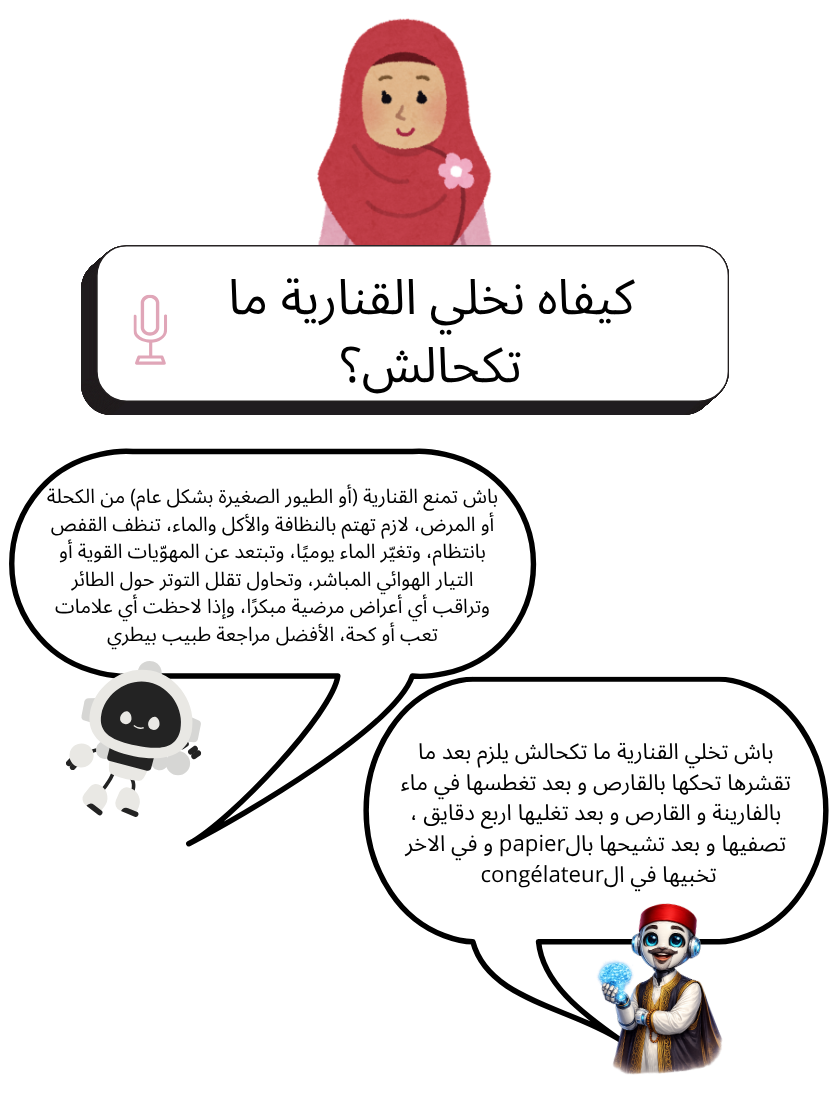
\includegraphics[width=0.6\linewidth]{fig1.png}
  \caption{Comparison of two responses to a spoken Tunisian Arabic culinary query}
    \label{fig:llm-eval-example}
\end{figure}
 % \textbf{``Kifeh nkhalli el ganaria ma tkahhalch?''} (How do I keep artichokes from
 %    turning dark?). The upper response, generated by GPT-4o, defaults to generic
 %    health-oriented advice about small birds (\textbf{ganaria} in MSA refers to a canary),
 %    illustrating a critical failure of dialectal disambiguation — the model maps the Tunisian
 %    term \textbf{ganaria} (artichoke) to its MSA homograph rather than inferring the correct
 %    culinary meaning from context. The lower response, representing the desired system
 %    behaviour, correctly identifies the ingredient and provides accurate, culturally grounded
 %    preparation instructions in authentic Tunisian Arabic, including natural code-switching
 %    with French culinary terms (\textbf{papier}, \textbf{congélateur}) consistent with
 %    everyday Tunisian speech. This example motivates the need for dialect-aware language
 %    models that ground lexical interpretation in Tunisian Arabic usage rather than MSA
 %    conventions.

%% =====================================================
% \section{Research Gap and Contributions}
% \label{sec:contributions}
% %% =====================================================

% Despite growing interest in Arabic dialect NLP, no existing work has fully evaluated and
% adapted both large language models and ASR systems for Tunisian Arabic within an integrated,
% end-to-end spoken dialogue framework. Prior research has addressed either ASR or text-based
% NLP in isolation, or has focused on better-resourced dialects such as Egyptian or Levantine
% Arabic. This work addresses that gap through the following contributions:

% \begin{enumerate}
%     \item \textbf{Curated Tunisian Arabic corpus and fine-tuning dataset.} We construct a
%           cleaned pretraining corpus of approximately 70~million tokens of Derja text, and
%           a culturally grounded question-answer dataset covering Tunisian proverbs,
%           culinary traditions, cinema, and dialect-specific knowledge, for use in
%           supervised fine-tuning.

%     \item \textbf{Dialect-adapted language model.} We adapt AYA-Expanse-8B to Tunisian
%           Arabic through continuous pretraining followed by supervised fine-tuning,
%           and augment the resulting model with a RAG knowledge base to support culturally
%           grounded generation at inference time.

%     \item \textbf{ASR adaptation for code-switched Tunisian speech.} We evaluate and
%           adapt Whisper-based ASR systems for dialectal and code-switched Tunisian Arabic,
%           addressing the phonetic, orthographic, and cross-lingual challenges specific to
%           this variety.

%     \item \textbf{End-to-end spoken dialogue system.} We integrate the adapted ASR and
%           LLM components into a unified pipeline and evaluate its end-to-end performance
%           on realistic Tunisian Arabic conversational tasks.
% \end{enumerate}

% Collectively, these contributions advance the computational modelling of a severely
% under-resourced dialect and demonstrate a replicable methodology for building spoken
% dialogue systems in similar low-resource settings. Beyond the immediate technical results,
% this work aims to support the development of digital tools and conversational interfaces
% that reflect the linguistic reality of millions of Tunisians — promoting both technological
% inclusivity and the preservation of dialectal identity in digital spaces.

% %% =====================================================
% \section{Report Organisation}
% \label{sec:organisation}
% %% =====================================================

% The remainder of this thesis is organised as follows. Chapter~\ref{chap:related} reviews
% related work on Arabic NLP, dialectal language modelling, low-resource ASR, and
% retrieval-augmented generation. Chapter~\ref{chap:data} describes the data collection,
% cleaning, and preparation methodology for both the pretraining corpus and the fine-tuning
% dataset. Chapter~\ref{chap:lm} presents the language model adaptation pipeline, covering
% continuous pretraining, supervised fine-tuning, and RAG integration.
% Chapter~\ref{chap:asr} details the ASR system adaptation for code-switched Tunisian speech.
% Chapter~\ref{chap:integration} evaluates the integrated spoken dialogue system on
% end-to-end tasks, and Chapter~\ref{chap:conclusion} concludes with a summary of findings
% and directions for future work.
% %% %% =====================================================
\chapter{Background \& Related Work}
\section{TunBERT: Pretrained Model for Tunisian Dialect}
TunBERT~\citep{messaoudi2021tunbertpretrainedcontextualizedtext} is one of the first transformer-based pretrained language models specifically developed for Tunisian Arabic. It was introduced to address a key limitation of multilingual models such as mBERT and XLM-R: despite their broad language coverage, they often struggle with low-resource dialects like Tunisian Arabic due to insufficient dialectal exposure during pretraining.
Tunisian Arabic differs significantly from Modern Standard Arabic (MSA), containing local vocabulary, informal grammar, borrowed French words, and frequent code-switching — features that generic Arabic models handle poorly.
TunBERT was trained on approximately 500,000 Tunisian dialect sentences collected from blogs, forums, and social media. A key finding is that a small but targeted corpus can outperform much larger generic ones when the target variety is highly specific.
The model was evaluated on three downstream tasks:
\begin{itemize}
\item Sentiment analysis
\item Tunisian dialect identification
\item Reading comprehension / Question answering
\end{itemize}
TunBERT outperformed multilingual baselines including mBERT and AraBERT, confirming that dialect-specific specialization can be more valuable than multilingual scale.
For this project, TunBERT is relevant as a tool to detect authentically Tunisian text, filter unnatural synthetic outputs, and support annotation pipelines for intent or sentiment labels.
\section{TounsiBench: Benchmark for Tunisian Arabic LLM Evaluation}
TounsiBench~\citep{hassine-etal-2025-tounsibench} is the first benchmark specifically designed to evaluate LLMs on Tunisian Arabic. It consists of 744 instructions paired with human-written references, spanning domains such as education, culture, finance, and technology. Outputs are assessed across four dimensions:
\begin{itemize}
\item Overall quality
\item Correctness
\item Relevance
\item Dialectal adherence
\end{itemize}
Results reveal a substantial gap between general LLM performance and Tunisian-specific capability. Common failure modes include dialect confusion with Moroccan or Algerian Arabic, drift toward MSA, poor code-switching handling, and unnatural vocabulary. GPT-4o achieved the strongest results, while open-source models showed inconsistent performance~\citep{benhassine2025tounsibench}.
These findings confirm that strong multilingual benchmarks scores do not transfer reliably to underrepresented dialects. TounsiBench is adopted here as the core evaluation framework for this project.
\section{TEDxTN}
TEDxTN introduced a three-way parallel corpus for code-switched Tunisian Arabic and English speech translation, built from TEDx talks across multiple Tunisian regions.
Its key contributions include:
\begin{itemize}
\item Accent and regional diversity
\item Formal spoken discourse
\item Parallel multilingual supervision
\end{itemize}
It reflects growing momentum toward multilingual spoken AI systems for Tunisian Arabic.
%%=====================================================
\chapter{ASR Fine-Tuning}
%% =====================================================

This chapter covers the full pipeline for building a fine-tuned Automatic Speech Recognition
system for Tunisian Arabic, following the CRISP-DM methodology. It spans data understanding,
data preparation, model selection, zero-shot benchmarking, and fine-tuning setup.

%% =====================================================
\section{Data Understanding}
%% =====================================================

\subsection{Dataset Overview}

The primary dataset used throughout this track is the publicly available
\textbf{LinTO Tunisian Arabic Speech Dataset}
(\texttt{linagora/linto-dataset-audio-ar-tn}), providing approximately \textbf{400 hours}
of real-world Tunisian Arabic speech. It is licensed under CC-BY 4.0 and hosted on
HuggingFace by LinAgora Research, France.

Key characteristics of the dataset include:

\begin{itemize}
    \item Spoken Tunisian Arabic from real-world scenarios with code-switched utterances
    (Arabic, French, English, Berber, Italian, Turkish).
    \item Corresponding human-verified transcriptions in mixed Arabic and Latin script.
    \item Audio segments of at most 30 seconds per sample.
    \item Target output constraint: Arabic script only — foreign spoken words must be
    transliterated, not left in Latin characters.
\end{itemize}

An augmented variant (\texttt{linto-dataset-audio-ar-tn-augmented}) exists and is planned
for a later extension of the pipeline once the base dataset processing is validated.

\subsection{Exploratory Audit}

An automated audit notebook (\textbf{Notebook 01 — Dataset Audit}) was executed to
characterise the raw data before any processing. It produced:

\begin{itemize}
    \item Descriptive statistics on audio duration distributions, sampling rates, and formats.
    \item Integrity checks flagging corrupted or misaligned audio-transcript pairs.
    \item Visualisations of segment length and language mixing patterns.
\end{itemize}

The audit confirmed the dataset is structurally sound but exhibits the variability expected
from real-world dialectal speech: inconsistent orthography, code-switching across multiple
languages, and non-standard transcription conventions that require normalisation before
training.

%% =====================================================
\section{Data Preparation}
%% =====================================================

The data preparation stage implements a four-notebook sequential pipeline. Each notebook
takes the outputs of the previous one as inputs, ensuring full traceability of the data flow.
The full pipeline runs in approximately \textbf{15 minutes} on a CPU-only environment
(24 GB RAM), with audio preprocessing representing 88.8\% of total execution time.

\subsection{Text Preprocessing}

\textbf{Notebook 02 — Text Preprocessing} applies a normalisation pipeline to produce
clean, consistent transcriptions conforming to NOTA/CODA standards. The main steps are:

\begin{itemize}
    \item \textbf{Unicode normalisation} and removal of diacritics and parasitic characters.
    \item \textbf{Orthographic unification} of common graphical variants while preserving
    dialectal characteristics.
    \item \textbf{Code-switching handling:} Latin-script tokens are detected and processed
    under a controlled policy — either arabised via transliteration, preserved, or removed
    depending on the token type.
    \item \textbf{NOTA-based normalisation} using a hierarchy of rules applied to
    non-standard forms.
    \item \textbf{Quality gate:} transcriptions failing conformity checks are logged and
    rejected rather than silently passed downstream.
\end{itemize}

\subsection{Audio Preprocessing}

\textbf{Notebook 03 — Audio Preprocessing} standardises all audio files to a uniform
format suitable for ASR model input:

\begin{itemize}
    \item Conversion to \textbf{mono channel} and resampling to \textbf{16 kHz}.
    \item Volume normalisation and removal of excessively silent segments.
    \item Export to a unified \textbf{WAV} format.
\end{itemize}

This notebook is the most computationally intensive step (approximately 13 minutes on CPU)
and is the primary candidate for GPU acceleration at larger scale.

\subsection{Dataset Construction}

\textbf{Notebook 04 — Dataset Builder} assembles the final dataset by aligning the
preprocessed audio files with their corresponding normalised transcriptions. It produces:

\begin{itemize}
    \item A structured \textbf{JSON/CSV manifest} pairing each audio segment with its
    transcript.
    \item Alignment and consistency checks on all pairs.
    \item Output in a format directly consumable by standard ASR training frameworks
    (HuggingFace, NeMo, Kaldi).
\end{itemize}

\subsection{Perspectives and Future Improvements}

Several improvements are planned for subsequent iterations of the pipeline:

\begin{itemize}
    \item \textbf{Full automation:} consolidating the four notebooks into a single end-to-end
    pipeline script with no manual intervention between stages.
    \item \textbf{Lexicon enrichment:} extending the code-switching handling tables to better
    cover acronyms, proper nouns, and technical terms.
    \item \textbf{Augmented dataset:} applying the validated pipeline to the
    \texttt{linto-dataset-audio-ar-tn-augmented} variant to expand training coverage.
\end{itemize}

%% =====================================================
\section{Modeling}
%% =====================================================
\subsection{Model Candidates and Selection Criteria}

A systematic review of available open-source ASR models was conducted to identify the
strongest candidates for zero-shot benchmarking on Tunisian and Algerian dialect data,
prior to fine-tuning selection. Ten models were evaluated against four criteria:
\textbf{Arabic and dialect coverage}, \textbf{architecture modernity and community support},
\textbf{inference efficiency} on available hardware, and \textbf{fine-tuning feasibility}.

\medskip
The key finding from zero-shot evaluation is unambiguous: \textbf{all evaluated models
achieve WER between 70\% and 140\% on the Linagora Tunisian corpus}, confirming that
fine-tuning on in-domain dialectal data is mandatory regardless of the chosen architecture.

\medskip
The Multilingual zero-shot candidate models are:

\begin{itemize}

  % \item \textbf{Baseline — Native Tunisian dialect model:}
  % \begin{itemize}
  %   \item \textbf{linagora/linto-asr-ar-tn-0.1} (LinAgora, undisclosed params, Apache 2.0,
  %   April 2025) --- The only open model natively targeting Tunisian Arabic, with partial
  %   French/English code-switching support. Built on a classical Kaldi TDNN acoustic model
  %   with an $n$-gram language model --- no Transformer or CTC component. Real-time capable
  %   via Vosk and WebRTC; edge-friendly Android variant available. Used as the reference
  %   ceiling for dialect-specific performance throughout this study.
  % \end{itemize}

  % \item \textbf{Multilingual zero-shot candidates:}

  \item \textbf{facebook/omniASR-LLM-7B-ZS} and CTC siblings (300M, 1B, 3B)
  \begin{itemize}
    \item \textbf{Origin \& coverage:} Meta, $\approx$7.81B params, Apache 2.0, November 2025.
    Covers 1,600+ languages including Tunisian Arabic (\texttt{aeb\_Arab}).
    \item \textbf{Architecture:} wav2vec2 encoder feeding an autoregressive Transformer decoder
    with a zero-shot generalisation head. CTC siblings share the same encoder and are designed
    for real-time deployment.
    \item \textbf{Key strengths:} Broadest dialect coverage of any evaluated model; official Meta
    fine-tuning recipe available; CTC siblings achieve sub-real-time RTF, making them viable
    for production deployment.
  \end{itemize}

  \item \textbf{facebook/mms-1b-all} with Arabic adapter
  \begin{itemize}
    \item \textbf{Origin \& coverage:} Meta, 1B params, CC-BY-NC 4.0, 2023.
    Covers 1,406 languages via swappable per-language adapter weights.
    \item \textbf{Architecture:} wav2vec2-based self-supervised encoder with language-specific
    adapter modules, enabling parameter-efficient inference and fine-tuning by swapping
    only the adapter layer.
    \item \textbf{Key strengths:} Arabic adapter available out-of-the-box; lowest adaptation
    cost of any evaluated model; Berber dialect variants also covered.
  \end{itemize}

  % \item \textbf{jonatasgrosman/wav2vec2-large-xlsr-53-arabic}
  % \begin{itemize}
  %   \item \textbf{Origin \& coverage:} Community fine-tune of XLSR-53, 317M params,
  %   Apache 2.0, 2021. Arabic only (fine-tuned from a 53-language checkpoint).
  %   \item \textbf{Architecture:} wav2vec2 large encoder with a CTC head fine-tuned
  %   end-to-end on Arabic Common Voice, enforcing Arabic-only output via a restricted
  %   CTC vocabulary — no language model component.
  %   \item \textbf{Key strengths:} Very lightweight and fast (RTF $\approx$ 0.02); natively
  %   enforces Arabic-only output; widely used as a community Arabic ASR baseline with
  %   extensive published evaluations.
  % \end{itemize}

  \item \textbf{CohereLabs/cohere-transcribe-03-2026}
  \begin{itemize}
    \item \textbf{Origin \& coverage:} Cohere, 2B params, Apache 2.0, March 2026.
    14 languages including Arabic (MSA).
    \item \textbf{Architecture:} Conformer encoder with a lightweight Transformer decoder,
    trained with cross-entropy on mel-spectrogram inputs. Supports vLLM and
    \texttt{torch.compile} for accelerated inference.
    \item \textbf{Key strengths:} Best-in-class accuracy for its size; up to $3\times$ faster
    inference than comparable models; automatic long-form audio chunking.
  \end{itemize}

  \item \textbf{mistralai/Voxtral-Mini-4B-Realtime-2602}
  \begin{itemize}
    \item \textbf{Origin \& coverage:} Mistral AI, 4B params (3.4B LM + 0.6B audio encoder),
    Apache 2.0, February 2026. 13 languages including Arabic (MSA).
    \item \textbf{Architecture:} Causal sliding-window audio encoder feeding a Ministral-3B
    LLM backbone, natively streaming via vLLM WebSocket API with configurable latency
    (80ms--2.4s).
    \item \textbf{Key strengths:} Sub-500ms true real-time streaming; supports sessions
    exceeding 3 hours on a single GPU ($\geq$16\,GB VRAM); strongest long-form streaming
    architecture among evaluated models.
  \end{itemize}

  \item \textbf{microsoft/VibeVoice-ASR}
  \begin{itemize}
    \item \textbf{Origin \& coverage:} Microsoft, 9B params (BF16), MIT, January 2026
    (updated March 2026). 51 languages including Arabic (MSA), French, and English with
    native code-switching support.
    \item \textbf{Architecture:} Speech-Augmented Language Model (SALM) combining a dual
    acoustic and semantic tokenizer that compresses audio at 7.5\,Hz into a 64K-token
    Qwen2.5 LLM context. Multiple output heads jointly produce speaker IDs, timestamps,
    and transcription in a single autoregressive pass.
    \item \textbf{Key strengths:} 60-minute single-pass inference without chunking; built-in
    speaker diarisation and timestamping; hotword injection for domain-specific vocabulary;
    official LoRA fine-tuning guide with vLLM support.
  \end{itemize}

  \item \textbf{Qwen/Qwen3-ASR-1.7B}
  \begin{itemize}
    \item \textbf{Origin \& coverage:} Alibaba, 1.7B params (BF16), Apache 2.0, April 2025
    (updated January 2026). 30 languages including Arabic (MSA) and 22 Chinese dialects.
    \item \textbf{Architecture:} Causal audio encoder feeding a Qwen3 LLM decoder, supporting
    unified streaming and offline inference within a single checkpoint. FlashAttention-2
    and vLLM compatible.
    \item \textbf{Key strengths:} State-of-the-art open-source accuracy, outperforming
    Whisper-large-v3 on standard benchmarks; compact 1.7B footprint with no separate
    streaming model required.
  \end{itemize}

  \item \textbf{openai/whisper-large-v3}
  \begin{itemize}
    \item \textbf{Origin \& coverage:} OpenAI, 1.55B params, MIT, late 2023.
    99 languages including Arabic.
    \item \textbf{Architecture:} Encoder--decoder Transformer trained with weak supervision
    on 5\,M hours of multilingual audio. Language output is forced via a decoder language
    token, natively constraining output to Arabic script. No streaming support.
    \item \textbf{Key strengths:} Largest fine-tuning community on HuggingFace; native
    Arabic-only output via language token; established reference across numerous Arabic
    ASR evaluation sets.
  \end{itemize}

  % \item \textbf{openai/whisper-large-v3-turbo}
  % \begin{itemize}
  %   \item \textbf{Origin \& coverage:} OpenAI, 809M params, MIT, 2024.
  %   99 languages including Arabic.
  %   \item \textbf{Architecture:} Pruned variant of Whisper large-v3 with a 4-layer decoder
  %   instead of 32, preserving the full encoder. Identical inference interface to large-v3,
  %   making it a drop-in replacement.
  %   \item \textbf{Key strengths:} Approximately $3\times$ faster than large-v3 with marginal
  %   accuracy cost; lowest memory footprint among the Whisper family; recommended for
  %   constrained GPU budgets.
  % \end{itemize}

\end{itemize}

\medskip
\subsection{Zero-Shot Benchmarking}

Before fine-tuning, a zero-shot evaluation was conducted to establish baseline performance
and confirm the model ranking on the target datasets.

\subsubsection*{Protocol}

All models were evaluated in zero-shot mode --- loaded with their original pre-trained weights
and applied directly to the evaluation splits with no task-specific adaptation.
Three evaluation sets were used:
\begin{itemize}
    \item \textbf{labeled\_linagora\_raw:} 2\,380--5\,482 samples, $\sim$3.2--6.0 hours of
    Tunisian Arabic speech with natural code-switching (Arabic, French, English).
    \item \textbf{labeled\_linagora\_cs\_arabize:} same samples as \texttt{raw} but with all
    French and English words transcribed using Arabic letters --- no Latin characters. This
    variant isolates the effect of script normalisation on model performance.
    \item \textbf{labeled\_algerian:} 400--500 samples, $\sim$3.2--4.0 hours of Algerian
    Arabic speech, used as a cross-dialect generalisation probe.
\end{itemize}

In addition, a manual evaluation was conducted on an unlabelled dataset of approximately
2 hours of YouTube videos in Tunisian dialect, providing an out-of-domain qualitative
assessment under real-world conditions.

Performance was measured using three metrics:
\begin{itemize}
    \item \textbf{WER (Word Error Rate):} proportion of word-level substitutions, deletions,
    and insertions relative to the reference. Values above 1.0 indicate more errors than
    reference words.
    \item \textbf{CER (Character Error Rate):} the same computation at the character level,
    more tolerant of partial matches and useful for Arabic script evaluation.
    \item \textbf{RTF (Real-Time Factor):} ratio of inference time to audio duration.
    Values below 1.0 indicate faster-than-real-time processing.
\end{itemize}

\subsubsection*{Results}

\begin{table}[H]
\centering
\small
\begin{tabular}{lrrrrrr}
\toprule
\multirow{2}{*}{\textbf{Model}} &
\multicolumn{3}{c}{\textbf{Tunisian} (\texttt{linagora\_raw})} &
\multicolumn{3}{c}{\textbf{Algerian}} \\
\cmidrule(lr){2-4} \cmidrule(lr){5-7}
& \textbf{WER} & \textbf{CER} & \textbf{RTF}
& \textbf{WER} & \textbf{CER} & \textbf{RTF} \\
\midrule
facebook/omniASR (CTC-7B)            & 0.6720 & 0.3470 & 0.036 & 0.9819 & 0.9063 & 0.028 \\
facebook/omniASR (CTC-3B)            & 0.6795 & 0.3470 & 0.024 & 0.9843 & 0.9224 & 0.011 \\
facebook/omniASR (CTC-1B)            & 0.6831 & 0.3456 & 0.014 & 0.9823 & 0.9010 & 0.007 \\
facebook/omniASR (CTC-300M)          & 0.7589 & 0.3843 & 0.008 & 0.9773 & 0.8696 & 0.005 \\
CohereLabs/cohere-transcribe-03-2026 & 0.7305 & 0.4405 & 0.064 & 1.0767 & 0.7769 & 0.050 \\
Qwen/Qwen3-ASR-1.7B                  & 0.7357 & 0.3448 & 0.227 & 0.9807 & 0.5584 & 0.185 \\
mistralai/Voxtral-Mini-4B            & 0.7541 & 0.4842 & 0.343 & 0.8715 & 0.6483 & 0.133 \\
facebook/mms-1b-all + Arabic adapter & 0.8492 & 0.4282 & 0.056 & 0.9369 & 0.5535 & 0.045 \\
jonatasgrosman/wav2vec2-xlsr-53-ar   & 0.9370 & 0.5322 & 0.024 & 0.9723 & 0.6061 & 0.021 \\
openai/whisper-large-v3              & 0.9692 & 0.6797 & 0.427 & 1.1153 & 0.7587 & 0.374 \\
openai/whisper-large-v3-turbo        & 1.4109 & 1.1183 & 0.164 & 1.3872 & 0.9483 & 0.045 \\
\bottomrule
\end{tabular}
\caption{Zero-shot results on Tunisian and Algerian splits, sorted by Tunisian WER.}
\label{tab:zero-shot-asr}
\end{table}

% \begin{table}[H]
% \centering
% \small
% \begin{tabular}{lrrrr}
% \toprule
% \multirow{2}{*}{\textbf{Model}} &
% \multicolumn{2}{c}{\textbf{raw}} &
% \multicolumn{2}{c}{\textbf{cs\_arabize}} \\
% \cmidrule(lr){2-3} \cmidrule(lr){4-5}
% & \textbf{WER} & \textbf{CER} & \textbf{WER} & \textbf{CER} \\
% \midrule
% facebook/omniASR (CTC-7B)            & 0.6720 & 0.3470 & 0.6790 & 0.3261 \\
% facebook/omniASR (CTC-3B)            & 0.6795 & 0.3470 & 0.6842 & 0.3249 \\
% facebook/omniASR (CTC-1B)            & 0.6831 & 0.3456 & 0.6906 & 0.3263 \\
% facebook/omniASR (CTC-300M)          & 0.7589 & 0.3843 & 0.7654 & 0.3610 \\
% CohereLabs/cohere-transcribe-03-2026 & 0.7305 & 0.4405 & 0.7138 & 0.4030 \\
% Qwen/Qwen3-ASR-1.7B                  & 0.7357 & 0.3448 & 0.7648 & 0.3419 \\
% mistralai/Voxtral-Mini-4B            & 0.7541 & 0.4842 & 0.7787 & 0.5043 \\
% facebook/mms-1b-all + Arabic adapter & 0.8492 & 0.4282 & 0.8562 & 0.3833 \\
% jonatasgrosman/wav2vec2-xlsr-53-ar   & 0.9370 & 0.5322 & 0.9405 & 0.4927 \\
% openai/whisper-large-v3              & 0.9692 & 0.6797 & 0.9735 & 0.6592 \\
% openai/whisper-large-v3-turbo        & 1.4109 & 1.1183 & 1.4144 & 1.1057 \\
% \bottomrule
% \end{tabular}
% \caption{Impact of Arabic script normalisation (\texttt{raw} vs \texttt{cs\_arabize})
% on Tunisian WER and CER.}
% \label{tab:arabize}
% \end{table}
\subsection{Analysis}

The zero-shot results reveal three distinct performance tiers among the evaluated models,
consistently observed across both evaluation splits.

\begin{itemize}

    \item \textbf{Top performers:}

    The \textbf{facebook/omniASR CTC family} (7B, 3B, 1B) forms a tight cluster on
    Tunisian data, with WER ranging from 0.672 (7B) to 0.683 (1B). All three variants
    achieve sub-real-time inference (RTF $\leq$ 0.036), with total processing times between
    310\,s (1B) and 787\,s (7B) on 6.0\,h of audio. This combination of competitive
    accuracy and fast inference makes them the primary candidates selected for fine-tuning.

    % The \textbf{CTC-300M} variant sits slightly outside this cluster (WER 0.7589) but
    % stands out for its exceptionally low RTF of 0.008 and a total inference time of only
    % 168\,s --- making it the most suitable option for edge and real-time deployment.

    \item \textbf{Mid-range models:}

    \textbf{CohereLabs/cohere-transcribe-03-2026} achieves a Tunisian WER of 0.7305 at a
    reasonable RTF of 0.064, while \textbf{Qwen/Qwen3-ASR-1.7B} reaches WER 0.7357 but
    at a significantly higher inference cost (RTF 0.227, total 2\,600\,s).

    \textbf{mistralai/Voxtral-Mini-4B} is the most computationally expensive model
    evaluated, requiring 7\,422\,s to process 6.0\,h of audio (RTF 0.343), which is over
    $9\times$ slower than the CTC-7B at comparable WER (0.7541 vs 0.6720). \newline Despite this
    cost, Voxtral achieves the best Algerian WER among all multilingual models (0.8715),
    suggesting stronger cross-dialect robustness that its Tunisian score alone does not
    reflect.

    \item \textbf{Underperforming models:}

    \textbf{facebook/mms-1b-all} with its Arabic adapter (WER 0.8492) and
    \textbf{wav2vec2-large-xlsr-53-arabic} (WER 0.9370) both show degraded performance.
    This is likely explained by the domain gap between their training corpora --- standard
    MSA or read Arabic speech --- and the spontaneous, code-switched Tunisian dialect of
    the Linagora corpus.

    \textbf{openai/whisper-large-v3} reaches WER 0.9692 and is the slowest model
    overall, requiring 9\,239\,s to process 6.0\,h of audio (RTF 0.427). Its pruned
    variant, \textbf{openai/whisper-large-v3-turbo}, performs worst on both evaluation
    splits with WER 1.4109 on Tunisian and WER 1.3872 on Algerian data --- producing more
    errors than reference words in both cases. This confirms that neither Whisper variant
    has meaningful prior exposure to Maghrebi dialect. Both are excluded from fine-tuning.

\end{itemize}

% \medskip
% \noindent\textbf{Script normalisation effect.}

% Arabization of code-switched tokens (Table~\ref{tab:arabize}) has a marginal and
% inconsistent impact on most models, with WER differences of $\leq$1\,pp in either
% direction. Three patterns emerge:

% \begin{itemize}
%     \item \textbf{CohereLabs/cohere-transcribe-03-2026} is the only model that benefits
%     clearly from arabization, gaining $-$1.7\,pp WER and $-$3.7\,pp CER. This suggests
%     its decoder is better calibrated for pure Arabic script and is penalised by the
%     presence of Latin characters in the reference.

%     \item \textbf{OmniASR CTC variants} (all four sizes) show a consistent pattern:
%     arabization marginally reduces CER while slightly increasing WER. Script normalisation
%     therefore improves character-level alignment without translating into word-level gains.

%     \item \textbf{All other models} (Qwen3, Voxtral, MMS, XLSR, Whisper) perform best
%     or equivalently on the raw mixed-script references, indicating that the presence of
%     Latin characters in the transcription does not penalise their output.
% \end{itemize}
\subsection{Fine-Tuning Setup}

Based on zero-shot results, \textbf{Whisper Large v3} and \textbf{w2v-BERT 2.0} are
prioritised for supervised adaptation on the prepared LinTO dataset. The fine-tuning
configuration is as follows:

\begin{itemize}
    \item \textbf{Method:} LoRA / QLoRA (parameter-efficient fine-tuning) to operate within
    student GPU constraints ($\leq$ 24 GB VRAM).
    \item \textbf{Training data:} the preprocessed LinTO manifest produced by the Data
    Factory pipeline, with possible extension to the augmented variant.
    \item \textbf{Transcript normalisation strategy:} Latin-script tokens in transcriptions
    will be either transliterated to Arabic phonetics (preferred, requires a transliteration
    dictionary) or stripped (fallback), ensuring Arabic-only decoder output.
    \item \textbf{Evaluation metrics:} WER and CER on a held-out test split, computed on
    Arabic-normalised references.
    \item \textbf{Target WER:} 25--40\% after fine-tuning, compared to 66--93\% in
    zero-shot settings on Maghrebi dialects.
\end{itemize}
%% =====================================================
%% ====================================================%% =====================================================
\chapter{LLM Adaptation for Tunisian Arabic}
%% =====================================================

This chapter presents a structured pipeline for adapting a large language model (LLM)
to understand and generate authentic Tunisian Arabic dialect. The approach is designed
for low-resource settings and follows a staged methodology.

%% =====================================================
\section{Pipeline Overview}
%% =====================================================

The proposed pipeline consists of seven stages, beginning with benchmarking open-source LLMs to identify the most suitable base model for Tunisian dialect adaptation.
\begin{table}[h]
\centering
\begin{tabular}{c l p{10cm}}
\toprule
\textbf{Stage} & \textbf{Name} & \textbf{Objective} \\
\midrule
1 & Open-Source LLM Benchmarking & Compare candidate open-source models \\
2 & Data Collection & Gather large-scale Tunisian dialect text \\
3 & Continued Pre-training & Adapt the selected model to Tunisian patterns \\
4 & Lexicon RAG Setup & Ground the model in Tunisian cultural knowledge \\
5 & Synthetic Data Generation & Create high-quality instruction--response data \\
6 & Supervised Fine-Tuning & Train instruction-following conversational behavior \\
7 & Final Evaluation & Measure fluency, dialect adherence, helpfulness \\
\bottomrule
\end{tabular}
\caption{Tunisian Dialect LLM Development Pipeline}
\end{table}
Each stage addresses a specific challenge of low-resource dialect modeling. Initial benchmarking ensures that adaptation starts from the strongest available open-source base model, while subsequent stages improve dialect knowledge, response quality, and real-world usability.


%% =====================================================
\section{Model Selection and Benchmarking}
%% =====================================================

\subsection{Candidate Models}

\begin{itemize}
    \item Llama-3.2-1B
    \item Llama-3-8B
    \item Labess-7B
    \item SILMA-9B
    \item Aya-Expanse-8B
\end{itemize}

\subsection{Zero-Shot Results}

\begin{table}[h]
\centering
\begin{tabular}{lcccc}
\toprule
Model & Quality & Correctness & Relevance & Dialect \\
\midrule
Aya-Expanse-8B & 1 & 2 & 2 & 0--1 \\
Labess-7B & 1 & 1 & 1 & 1 \\
SILMA-9B & 1 & 1--2 & 1--2 & 0 \\
Llama-3-8B & 1 & 1 & 1 & 0 \\
Llama-3.2-1B & 0 & 0--1 & 0 & 0 \\
\bottomrule
\end{tabular}
\caption{Zero-shot evaluation results}
\end{table}

\subsection{Key Findings}

\begin{itemize}
    \item All models fail on dialect adherence
    \item Aya-Expanse-8B is the best fine-tuning candidate
    \item Fine-tuning is mandatory for dialect generation
\end{itemize}% =====================================================

% =====================================================

\section{Data Collection and Understanding}

% =====================================================
\subsection{Challenges}

Tunisian Arabic (Derja) presents several inherent difficulties for corpus construction
and language modelling:

\begin{itemize}
    \item \textbf{No standardized orthography.} Tunisian Arabic lacks a codified
          written standard, resulting in high intra-speaker and inter-speaker spelling
          variability for the same lexical item (e.g.\ \ \ar{باش} vs.\ \ \ar{بش} both appear
          frequently in the corpus with cumulative frequencies exceeding 700{,}000
          occurrences).

    \item \textbf{Code-switching.} Social-media text routinely mixes Tunisian Arabic
          with French, English, and occasionally Berber. Script-level analysis of the
          collected data reveals that 5.18\% of samples are \emph{mixed-script}
          (Arabic + Latin), requiring explicit filtering to prevent script noise from
          propagating into the training set.

    \item \textbf{MSA contamination.} Modern Standard Arabic (MSA) tokens and
          constructions co-occur with dialectal text, blurring the boundary between
          the target register and the high-resource variety.

    \item \textbf{Scarcity of labelled data.} Supervised resources for Tunisian Arabic
          remain sparse; most available datasets are small, domain-specific, or lack
          consistent annotation guidelines.
\end{itemize}

% =====================================================
\subsection{Data Sources}

The corpus was constructed by aggregating multiple Tunisian dialect datasets
from the Hugging Face Hub, complemented by the Linagora Tunisian Derja
collection \citep{linagora2025LLM-tn}. This multi-source strategy ensures diversity in linguistic styles,
domains, and annotation types. After collection, filtering, and normalization,
all selected resources were unified into a single consolidated dataset and
published on Hugging Face under
\texttt{Syrinesmati/tunisian-dialect-corpus}
\citep{tunisian_dialect_corpus_cleaned_2026}.

\begin{itemize}

    \item \textbf{\texttt{atakaboudi/Dialect\_of\_Tunisia-Work\_Collection}}:
    This repository consolidates a wide range of Tunisian NLP datasets into a
    unified corpus designed for diverse downstream applications. The data
    exclusively consists of Tunisian Arabic written in Arabic script, with
    frequent code-switching involving French, English, and Italian. The
    collection represents approximately 70 million GPT-4 tokens
    \citep{abdallah2023leveraging}.

    It integrates the following datasets:

    \begin{itemize}

        \item \textbf{\texttt{Arbi-Houssem/Tunisian\_dataset\_STT-TTS15s\_filtred\_organiser\_Mixed}}:
        A speech-to-text dataset; transcripts are preserved without modification
        \citep{arbi_houssem_stt_tts}.

        \item \textbf{\texttt{linagora/linto-asr-ar-tn-0.1}}:
        An automatic speech recognition (ASR) dataset combining multiple sources,
        including \textbf{Youtube\_TNScrapped}, \textbf{TunswitchTO},
        \textbf{TunswitchCS}, \textbf{ApprendreLeTunisien}, \textbf{Taric}, and
        \textbf{OneStory}. All sentences are retained in their original form
        \citep{linagora2024Linto-tn,linagora2024linto_asr}.

        \item \textbf{Tunisian Arabic Dialects Identification (TADI)}:
        A binary classification dataset used to distinguish Tunisian dialect from
        other Arabic dialects. Only samples labeled as Tunisian are retained
        \citep{tadi}.

        \item \textbf{Tunisian Algerian Dialect (TAD)}:
        A dataset for distinguishing Tunisian from Algerian dialect. Only
        Tunisian-labeled samples are included \citep{tunbert_tad}.

        \item \textbf{\texttt{khaled123/tunninjaar}}:
        A dataset extracted from the Derja Ninja platform
        \citep{tunninjaar}.

        \item \textbf{T-HSAB — Tunisian Hate Speech and Abusive Dataset}:
        A dataset annotated for hate speech detection. Only non-hate-speech
        samples are retained to ensure neutral language modeling
        \citep{mulki2019tsab}.

        \item \textbf{Tunisian Reading Comprehension Dataset}:
        A question-answering dataset based on a dialectal adaptation of the
        Tunisian constitution. It contains 144 documents, each composed of three
        paragraphs, with three question--answer pairs per paragraph
        \citep{tunisian_rc}.

        \item \textbf{Naim Mhedhbi Tunisian Dialect Corpus v0}:
        A collection of 40{,}000 Facebook comments labeled by sentiment.
        Only positive and neutral samples are retained
        \citep{mhedhbi_tunisian_v0}.

        \item \textbf{TSAC — Tunisian Sentiment Analysis Corpus}:
        A dataset of approximately 17{,}000 annotated Facebook comments for
        sentiment analysis \citep{tsac}.

        \item \textbf{\texttt{khaled123/Testtun}} and
        \textbf{\texttt{khaled123/Tuniset}}:
        Additional Tunisian dialect datasets scraped from social media platforms
        incorporated to further increase lexical and stylistic diversity
        \citep{testtun,tuniset}.

        \item \textbf{\texttt{khaled123/Tunisian\_English\_dialectic\_Derja}}:
        A bilingual Tunisian-English dialect dataset included to enrich lexical
        variation and code-switching patterns
        \citep{Tunisian_English_dialectic_Derja}.

    \end{itemize}

\end{itemize}

        \begin{table}[h]
\centering
\caption{Token distribution across datasets in the aggregated corpus}
\label{tab:token_distribution}
\begin{tabular}{l r}
\hline
\textbf{Dataset} & \textbf{Token Count} \\
\hline
arbi\_houssem-tunisian-dataset\_stt\_tts15s\_filtered1.0 & 129{,}207 \\
maal-32173-Tunisian\_Revolution\_Arabic-2011-2022 & 11{,}538{,}264 \\
TAD & 41{,}434 \\
TADI & 891{,}750 \\
testtun-khaldoun & 18{,}356{,}271 \\
thsab & 289{,}310 \\
ts-naim-mhedhbi & 224{,}434 \\
tsac & 97{,}085 \\
tuninjar & 13{,}056{,}137 \\
tuniset & 22{,}584{,}964 \\
linagoraSTT & 2{,}003{,}450 \\
\hline
\textbf{Total} & \textbf{69{,}422{,}659} \\
\hline
\end{tabular}
\end{table}

\begin{itemize}
\item \textbf{Linagora Tunisian Derja Dataset}:
This dataset is a large-scale collection of Tunisian dialect textual data
designed for language modeling. It was notably used for the continual
pre-training of the JAIS large language model on Tunisian Arabic.
\end{itemize}
The corpus covers multiple domains, including social media, sentiment analysis,
code-switching, and dialectal variations. It is composed of 12 configurations:


\begin{itemize}
    \item \texttt{Derja\_tunsi}
    \item \texttt{MADAR\_TunisianDialect}
    \item \texttt{QADI\_TunisianDialect}
    \item \texttt{HkayetErwi}
    \item \texttt{Sentiment\_Derja}
    \item \texttt{TA\_Segmentation}
    \item \texttt{TSAC}
    \item \texttt{TuDiCOI}
    \item \texttt{TunSwitchTunisiaOnly}
    \item \texttt{TunisianSentimentAnalysis}
    \item \texttt{Tunisian\_Dialectic\_English\_Derja}
    \item \texttt{Tweet\_TN}
\end{itemize}

Table~\ref{tab:derja_distribution} summarizes the number of lines per subset.

\begin{table}[h]
\centering
\caption{Line distribution across the Linagora Tunisian Derja Dataset subsets}
\label{tab:derja_distribution}
\begin{tabular}{l r}
\hline
\textbf{Subset} & \textbf{Number of Lines} \\
\hline
Tunisian\_Dialectic\_English\_Derja & 1{,}220{,}712 \\
HkayetErwi & 946 \\
Derja\_tunsi & 13{,}037 \\
TunBERT & 67{,}219 \\
TunSwitchCodeSwitching & 394{,}163 \\
TunSwitchTunisiaOnly & 380{,}546 \\
Tweet\_TN & 39{,}637 \\
TSAC & 8{,}416 \\
TuDiCOI & 3{,}426 \\
Sentiment\_Derja & 22{,}890 \\
TA\_Segmentation & 30{,}530 \\
TunisianSentimentAnalysis & 23{,}786 \\
QADI\_TunisianDialect & 8{,}879 \\
MADAR\_TunisianDialect & 12{,}000 \\
\hline
\textbf{Total} & \textbf{1{,}764{,}805 } \\
\end{tabular}
\end{table}
\noindent This dataset provides a rich mixture of dialectal variation, sentiment
annotation, and code-switched text, making it particularly suitable for robust
language modeling in Tunisian Arabic.

\noindent The resulting aggregated corpus contains a total of
\textbf{2,057,757 samples} prior to preprocessing and cleaning.
% =====================================================
\subsection{Exploratory Data Analysis}
% =====================================================

\subsubsection{Dataset Overview}

The aggregated corpus consists of \textbf{2,057,757 samples}, providing a substantial resource for modeling Tunisian Arabic in a low-resource setting. Within this corpus, \textbf{63,527 samples} contain numerical tokens, representing approximately 3\% of the data.

The relatively low proportion of numerical content suggests that such tokens are not a dominant linguistic feature of the dataset. Nevertheless, they may introduce heterogeneity in token distributions (e.g., dates, prices, identifiers) and are therefore explicitly considered during preprocessing.

% -----------------------------------------------------

\subsubsection{Language and Script Distribution}

The distribution of languages and scripts within the corpus is highly imbalanced:

\begin{itemize}
    \item \textbf{Arabic:} 1,929,420 samples (\(\sim 93.7\%\))
    \item \textbf{Mixed (Arabic + Latin):} 123,315 samples (\(\sim 6\%\))
    \item \textbf{French:} 2,677 samples
    \item \textbf{Other:} 2,345 samples
\end{itemize}

The predominance of Arabic-script content confirms that the dataset is well-aligned with the target linguistic domain. However, the presence of mixed-script samples reflects widespread \textbf{code-switching}, a salient feature of Tunisian Arabic, particularly in informal and user-generated content.

The marginal proportion of purely French and other-language samples indicates limited cross-lingual contamination; these samples are treated as noise and excluded during preprocessing to preserve linguistic consistency.

% -----------------------------------------------------

\subsubsection{Length Distribution Analysis}

To characterize the structural properties of the corpus, we analyze both word-level and character-level length distributions.

\paragraph{Word Count Distribution}

The distribution of word counts exhibits a pronounced \textbf{right-skewed (long-tail)} behavior, indicating that the majority of samples are short, while a small fraction consists of significantly longer sequences.

\begin{figure}[H]
    \centering
    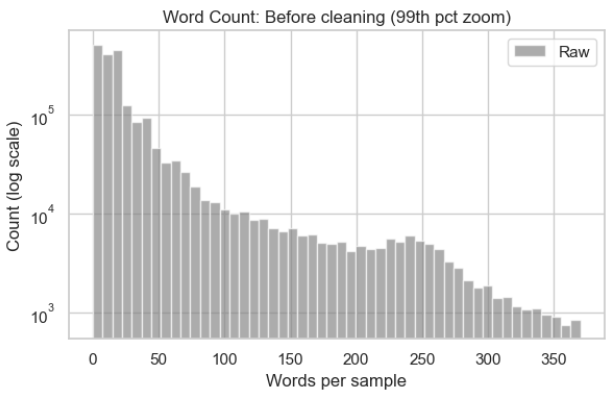
\includegraphics[width=0.5\linewidth]{image5.png}
    \label{fig:word_length_distribution}
\end{figure}

The empirical 99th percentile is estimated at
\textbf{370 words per sample}

This suggests that the corpus is largely composed of short-form textual units, such as conversational utterances or social media posts, which are particularly suitable for dialogue modeling and generative tasks.

\paragraph{Character Length Distribution}

A consistent trend is observed at the character level.

\begin{figure}[H]
    \centering
    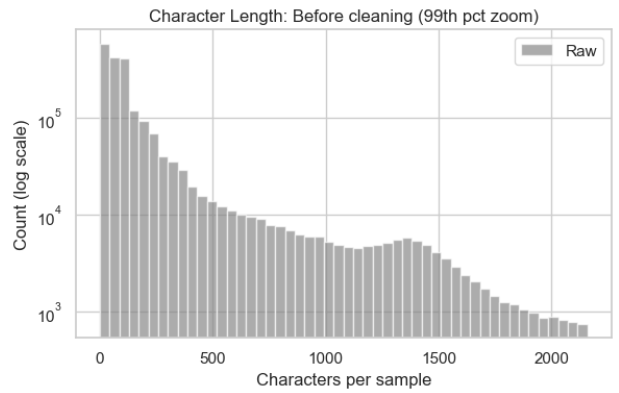
\includegraphics[width=0.5\linewidth]{image6.png}
    \label{fig:character_length_distribution}
\end{figure}

The 99th percentile of the character length distribution is \textbf{2159 characters per sample}


This further corroborates the predominance of compact textual samples, with a limited number of extreme-length instances.

% -----------------------------------------------------

\subsubsection{Outlier Analysis}

The long-tail distributions observed at both word and character levels indicate the presence of outliers in the form of unusually long samples. Such instances can negatively impact training efficiency and model performance by:

\begin{itemize}
    \item Increasing memory and computational requirements
    \item Introducing inefficiencies due to excessive padding
    \item Potentially biasing the model toward atypical sequence structures
\end{itemize}

To mitigate these effects, sequence length constraints are imposed based on high-percentile thresholds (e.g., 99th percentile), ensuring a balance between data retention and computational efficiency.

% -----------------------------------------------------

\subsubsection{Implications for Preprocessing}

The findings of this exploratory analysis directly inform the design of the preprocessing pipeline:

\begin{itemize}
    \item \textbf{Length filtering:} Sequences exceeding 370 words (or approximately 2000 characters) are truncated or discarded to control variance and computational cost.
    \item \textbf{Language filtering:} Non-Arabic samples are removed to maintain domain consistency.
    \item \textbf{Code-switching handling:} Mixed-script samples are either normalized or selectively retained, depending on their relevance to downstream tasks.
    \item \textbf{Numeric normalization:} Numerical tokens are standardized or removed to reduce token-level sparsity.
\end{itemize}

% =====================================================
\subsection{Data Cleaning Pipeline}
% =====================================================

The preprocessing stage is designed to ensure high-quality, linguistically consistent data for downstream language modeling tasks. Given the noisy nature of user-generated content in Tunisian Arabic (e.g., social media text, informal conversations), a multi-stage cleaning pipeline is employed to normalize, filter, and structurally refine the corpus.

The pipeline operates in a sequential manner, combining rule-based normalization, heuristic filtering, and redundancy elimination techniques.

% -----------------------------------------------------

\subsubsection{Text Normalization}

The initial stage focuses on standardizing raw text by removing extraneous elements that do not contribute to semantic content. This includes:

\begin{itemize}
    \item \textbf{Emoji removal:} All Unicode emoji ranges are stripped to reduce non-linguistic noise.
    \item \textbf{Special pattern filtering:} Structural artifacts such as brackets, audio markers (e.g., \textbf{[ضحك]}), transcription annotations, and platform-specific tokens (e.g., RT, AFP, instruction markers) are removed.
    \item \textbf{Whitespace normalization:} Multiple spaces are collapsed into a single space, and leading/trailing spaces are trimmed.
    \item \textbf{Symbol filtering:} Non-Arabic symbols are removed while preserving Arabic script and essential punctuation.
\end{itemize}

This stage ensures that the resulting text is structurally clean while preserving linguistic information.

% -----------------------------------------------------

\subsubsection{Language and Script Filtering}

To maintain dataset homogeneity, a strict script-level filtering strategy is applied. Each sample is classified into one of four categories: Arabic, mixed (Arabic–Latin), French, or other.

Samples containing Latin-script content are removed at the document level rather than partially cleaned, in order to avoid preserving noisy code-switched fragments. Similarly, non-Arabic samples (French and others) are discarded due to their negligible proportion and limited relevance to the target domain.

% -----------------------------------------------------

\subsubsection{Noise and Pattern-Based Filtering}

To further enhance data quality, heuristic rules are applied to remove linguistically noisy samples:

\begin{itemize}
    \item \textbf{Numerical filtering:} Entries containing numeric tokens are excluded to reduce heterogeneity introduced by dates, prices, and identifiers.
    \item \textbf{Hashtag removal:} Social media hashtags are filtered out as they introduce non-standard lexical units.
    \item \textbf{Character repetition filtering:} Samples containing excessive character elongation (e.g., expressive repetitions) are removed.
    \item \textbf{Word repetition filtering:} Instances of consecutive repeated words are discarded.
    \item \textbf{Lexical dominance filtering:} Samples in which a single token dominates more than 50\% of the text are considered degenerate and removed.
\end{itemize}

These heuristics are particularly important for social media corpora, where informal writing styles introduce substantial noise.

% -----------------------------------------------------

\subsubsection{Deduplication Strategy}

Redundancy reduction is performed using a two-level deduplication process:

\begin{itemize}
    \item \textbf{Exact deduplication:} Removal of identical samples.
    \item \textbf{Near-duplicate detection:} Normalization-based matching is applied using a canonical representation of text, which accounts for:
    \begin{itemize}
        \item Diacritic removal
        \item Normalization of Arabic letter variants
        \item Punctuation stripping
        \item Whitespace normalization
    \end{itemize}
\end{itemize}

This step mitigates data leakage and prevents overrepresentation of semantically equivalent samples.

% -----------------------------------------------------

\subsubsection{Length-Based Filtering}

To control sequence variability and computational cost, length-based constraints are enforced:

\begin{itemize}
    \item Very short texts are removed based on a minimum character and word threshold.
    \item Extremely long sequences are implicitly constrained through earlier statistical analysis (99th percentile thresholds).
\end{itemize}

This ensures a balanced distribution of sequence lengths suitable for training transformer-based models.

% -----------------------------------------------------

\subsubsection{Final Standardization and Annotation}

In the final stage, the dataset is standardized and enriched with auxiliary annotations:

\begin{itemize}
    \item Column normalization (standardizing text field naming).
    \item Script classification (Arabic, mixed, French, other).
    \item Length feature extraction (word and character counts).
\end{itemize}

These metadata fields facilitate downstream analysis and dataset stratification.

% =====================================================
% =====================================================
\subsection{Token Count}

The cleaned corpus was tokenised with the
\textbf{CohereLabs/aya-expanse-8b} tokeniser (BPE, multilingual).
The total token count on the final 1{,}616{,}232-sample split is:

\begin{equation}
    N_{\text{tokens}} = 150{,}459{,}946 \approx 150\text{M tokens}
\end{equation}

\noindent This exceeds the initial target range of 50--100M tokens, confirming
that the assembled corpus provides sufficient scale for Stage~1 continual
pre-training.
%% =====================================================
\section{Continued Pre-Training}

%% =====================================================
\subsection{Objective}

The objective of this phase is to adapt the base multilingual model to the
Tunisian Arabic dialect by exposing it to large amounts of raw dialectal text.
Although the chosen base model, Aya Expanse 8B, was pre-trained on 23
languages including Modern Standard Arabic and French --- both of which
strongly influence Tunisian dialect --- it was never explicitly trained on
Tunisian dialectal data. Continued Pre-Training (CPT) bridges this gap by
updating the model's internal representations to better capture the vocabulary,
morphology, code-switching patterns, and writing conventions specific to
Tunisian Arabic, without discarding the rich multilingual knowledge already
encoded in the model.

%% =====================================================
\subsection{Methodology}

Rather than training a language model from scratch, which would require
prohibitive computational resources and massive amounts of data, we applied
Continued Pre-Training: the base model is initialized with its original
pre-trained weights, and training is resumed on a domain-specific corpus using
the standard causal language modelling objective. The model is trained to
predict the next token in a sequence, which forces it to internalize the
statistical patterns of the new dialect.

To make training feasible on available hardware, we adopted the
\textbf{QLoRA} paradigm \cite{dettmers2023qlora}, which combines two
complementary efficiency techniques:

\begin{itemize}
    \item \textbf{4-bit quantization (NF4):} The base model weights are
    quantized to 4-bit Normal Float precision using double quantization,
    reducing GPU memory consumption by approximately 75\% compared to
    full-precision loading, while preserving model quality through a
    \texttt{bfloat16} computation dtype.

    \item \textbf{Low-Rank Adaptation (LoRA):} Instead of updating all 8
    billion parameters of the base model, small trainable rank-decomposition
    matrices are injected into the key projection layers of the Transformer
    architecture. Only these adapter weights are updated during training,
    drastically reducing the number of trainable parameters while still
    allowing meaningful adaptation. The LoRA adapters were applied to all
    attention and feed-forward projection layers: \texttt{q\_proj},
    \texttt{k\_proj}, \texttt{v\_proj}, \texttt{o\_proj}, \texttt{gate\_proj},
    \texttt{up\_proj}, and \texttt{down\_proj}.
\end{itemize}

This combination allowed us to fine-tune an 8B parameter model on a single
GPU with a memory footprint comparable to a much smaller model.

%% =====================================================
\subsection{Experimental Setup}

\subsubsection{Hardware}

Training was conducted on a single \textbf{NVIDIA GB10 GPU} with
\textbf{124 GB of VRAM}. The full training run completed in approximately
\textbf{75 hours}, of which roughly 70 hours were spent on forward and
backward passes, and approximately 5 hours on periodic evaluation. At the
observed throughput of $\sim$71 optimizer steps per hour (one step every
$\sim$51 seconds), the total compute amounted to approximately
$3.53 \times 10^{18}$ floating-point operations (FLOPs).

\subsubsection{Data Preparation and Tokenization}

The training corpus is the Tunisian Dialect Corpus
(\texttt{Syrinesmati/tunisian-dialect-    corpus}) with 1,18 million rows and 85 million tokens. After filtering out all null
or empty entries, the cleaned dataset was tokenized using the Aya Expanse
tokenizer. The resulting token sequences were then packed into fixed-length
blocks of \textbf{1,024 tokens} using a concatenation-and-chunking strategy:
all token sequences are first concatenated into a single long stream, which is
then split into consecutive non-overlapping chunks of exactly 1,024 tokens.
Any remainder that does not fill a complete block is discarded. This packing
strategy ensures that every training example is fully dense, eliminating
padding tokens entirely and maximizing GPU utilization.

After packing, the resulting dataset contained \textbf{82,634 blocks},
representing approximately \textbf{84.6 million tokens} in total. This was
split into a training set of \textbf{81,808 blocks} (99\%) and an evaluation
set of \textbf{826 blocks} (1\%), used to monitor generalization throughout
training.

\subsubsection{Step Count Derivation}

The total number of optimizer steps is determined by the following formula:

\begin{equation}
    N_{\text{steps}} = \left\lfloor \frac{N_{\text{train}}}{B_{\text{eff}}}
    \right\rfloor \times E
\end{equation}

\noindent where $N_{\text{train}} = 81{,}808$ is the number of training
blocks, $B_{\text{eff}} = 16$ is the effective batch size (1 sample per device
$\times$ 16 gradient accumulation steps), and $E = 1$ is the number of epochs.
This yields:

\begin{equation}
    N_{\text{steps}} = \left\lfloor \frac{81{,}808}{16} \right\rfloor = 5{,}113
    \text{ optimizer steps}
\end{equation}

\subsubsection{Checkpointing and Evaluation Strategy}

A checkpoint was saved every \textbf{200 steps}, resulting in \textbf{25
checkpoint saves} over the full training run. To manage disk space, only the
\textbf{3 most recent checkpoints} were retained at any time
(\texttt{save\_total\_limit = 3}), with earlier ones being automatically
deleted. This setup also enables seamless training resumption in case of
interruption, as the trainer automatically detects and resumes from the latest
available checkpoint.

Evaluation on the held-out set was performed with the same frequency,
every \textbf{200 steps}, for a total of \textbf{26 evaluation passes}
(including a final evaluation at the end of the epoch). Each evaluation pass
took approximately 680 seconds on average, processing the 826 evaluation
blocks.

\subsubsection{Hyperparameters}

The key training hyperparameters are summarized in Table~\ref{tab:cpt_hparams}.

\begin{table}[h]
\centering
\caption{CPT Hyperparameters}
\label{tab:cpt_hparams}
\begin{tabular}{ll}
\toprule
\textbf{Hyperparameter} & \textbf{Value} \\
\midrule
Base model              & CohereLabs/aya-expanse-8b \\
Training objective      & Causal Language Modelling \\
Epochs                  & 1 \\
Sequence length         & 1,024 tokens \\
Total training tokens   & $\approx$ 84.6 million \\
Training blocks         & 81,808 \\
Evaluation blocks       & 826 \\
Learning rate           & $2 \times 10^{-4}$ \\
LR scheduler            & Cosine decay \\
Warmup ratio            & 3\% ($\approx 153$ steps) \\
Optimizer               & Paged AdamW 8-bit \\
Batch size (per device) & 1 \\
Gradient accumulation   & 16 steps \\
Effective batch size    & 16 \\
Total optimizer steps   & 5,113 \\
Checkpoint frequency    & Every 200 steps \\
Evaluation frequency    & Every 200 steps \\
Checkpoints retained    & 3 (rolling) \\
Quantization            & 4-bit NF4 (double quantization) \\
LoRA rank ($r$)         & 16 \\
LoRA alpha ($\alpha$)   & 32 \\
LoRA dropout            & 0.05 \\
LoRA target modules     & All attention \& MLP projections \\
GPU                     & NVIDIA GB10 (124 GB VRAM) \\
Training duration       & 75 hours \\
\bottomrule
\end{tabular}
\end{table}

%% =====================================================
\subsection{Results and Analysis}

Training ran for one full epoch over the corpus, completing 5,113 optimizer
steps. The evolution of the training and evaluation loss is reported at
representative checkpoints in Table~\ref{tab:cpt_loss}.

\begin{table}[h]
\centering
\caption{CPT Loss Progression at Representative Checkpoints}
\label{tab:cpt_loss}
\begin{tabular}{ccc}
\toprule
\textbf{Step} & \textbf{Train Loss} & \textbf{Eval Loss} \\
\midrule
25      & 3.633 & ---   \\
200     & 2.558 & 2.553 \\
600     & 2.402 & 2.367 \\
1{,}000 & 2.316 & 2.292 \\
1{,}800 & 2.236 & 2.210 \\
2{,}600 & 2.156 & 2.153 \\
3{,}400 & 2.130 & 2.115 \\
4{,}200 & 2.088 & 2.094 \\
5{,}000 & 2.081 & 2.089 \\
5{,}113 & 2.105 & 2.089 \\
\bottomrule
\end{tabular}
\end{table}

\noindent\textbf{Note: step 25 has no evaluation loss because evaluation was
only triggered every 200 steps. Step 5,113 is the final step of the epoch;
its training loss is the last logged value at step 5,100 (2.105), and its
evaluation loss is the final end-of-epoch evaluation.}

Several observations can be drawn from these results:

\begin{itemize}
    \item \textbf{Significant loss reduction:} The training loss dropped from
    3.633 at the very first logging step to 2.081 by the end of training, and
    the evaluation loss converged to \textbf{2.089}. This substantial decrease
    of approximately 1.54 nats confirms that the model successfully internalized
    the statistical patterns of the Tunisian dialect over the course of
    training.

    \item \textbf{No overfitting:} Throughout all 26 evaluation passes, the
    training and evaluation losses remained closely aligned, with a gap never
    exceeding 0.01 at any checkpoint. This indicates that the model generalized
    well to unseen dialectal text rather than memorizing the training corpus,
    which is the expected and desirable behaviour for a CPT phase.

    \item \textbf{Stable convergence:} The loss curve followed a smooth and
    monotonically decreasing trajectory. The cosine learning rate schedule
    contributed to this stability, decaying gracefully from $2 \times 10^{-4}$
    during the main training phase to near zero in the final steps. No
    instability, loss spikes, or divergence were observed at any point.

    \item \textbf{Stable optimization dynamics:} The gradient norms remained
    consistently in the range of 0.38--0.47 throughout all 5,113 steps,
    confirming well-behaved optimization with no signs of exploding or
    vanishing gradients.
\end{itemize}

The final adapted model was saved and published at:
\begin{center}
\url{https://huggingface.co/alabenayed/improved-aya-expanse-8b-cpt-tunisian}
\end{center}

This checkpoint serves as the foundation for the subsequent Supervised
Fine-Tuning (SFT) phase, where the model will be further specialized for
downstream Tunisian Arabic NLP tasks.


\section{Supervised Fine-Tuning}

%% =====================================================
\subsection{Objective}

The objective of this phase is to transform the dialect-adapted language model
produced by CPT into a structured, instruction-following assistant. While CPT
taught the model \emph{how Tunisian Arabic sounds}, it did not teach it
\emph{how to behave}: the model had no notion of questions, answers, roles, or
conversational structure. Supervised Fine-Tuning (SFT) addresses this by
training the model on curated question--response pairs formatted as
multi-turn conversations, conditioning it to produce helpful, on-topic, and
appropriately sized responses in Tunisian dialect.

A key design decision was to give the model a named identity:
\textbf{``التيجاني''} (Al-Tijani), a Tunisian AI assistant persona defined to
respond exclusively in Tunisian Darija, to calibrate response length to the
complexity of the question, and to resist hallucination and topic drift. This
persona is injected as a system prompt at the start of every training example.

%% =====================================================
\subsection{Methodology}

SFT continues directly from the CPT checkpoint
(\texttt{alabenayed/improved-aya-expanse        -8b-cpt-tunisian}), loading it as a
PEFT adapter on top of the Aya Expanse 8B base model. The adapter weights
remain trainable, so the SFT phase refines the same LoRA parameters that were
adapted during CPT, deepening dialect specialisation while simultaneously
learning conversational structure.

A critical distinction from CPT is the use of \textbf{assistant-only loss}.
In standard language modelling, the loss is computed over every token in the
sequence, including the system prompt and the user's question. This is
undesirable for SFT: we do not want the model to learn to predict the user's
input, only to produce good assistant responses. To enforce this, the tokenizer chat template was patched to include a
\verb|{% generation %}| marker, which signals to TRL's \texttt{SFTTrainer}
the exact boundary at which loss computation should begin. Only tokens belonging to the assistant's reply
contribute to the gradient, making training more targeted and sample-efficient.

Each training example is formatted as a three-turn conversation: a
\textbf{system} turn carrying the "tijani" persona prompt, a \textbf{user}
turn carrying the question, and an \textbf{assistant} turn carrying the target
response --- the only part over which loss is computed. Each row was rendered
to a flat text string via \texttt{tokenizer.apply\_chat\_template} using the
model's native chat template.

Unlike CPT, which required 4-bit quantization to fit the model in memory, the
SFT phase was conducted in \textbf{full bfloat16 precision} with no
quantization. The complete model (base weights + LoRA adapter) resided in
memory at native precision, which improves gradient quality and training
stability. The optimizer used was \texttt{adamw\_torch\_fused}, a
high-performance fused AdamW implementation suited for bf16 training, with a
weight decay of 0.01.

%% =====================================================


\subsection{Setup}

Training was conducted on the same \textbf{NVIDIA GB10 GPU} with \textbf{124
GB of VRAM}. The SFT dataset is
\texttt{Syrinesmati/tunisian-question-response-dataset}, a curated collection
of Tunisian Arabic question--response pairs with pre-defined \texttt{train} and
\texttt{test} splits. The training split contains \textbf{25,344 examples}.
Over the full 2-epoch run, the model processed approximately \textbf{9.59
million assistant tokens} (loss-bearing tokens only).

The effective batch size was 32 (8 samples per device $\times$ 4 gradient
accumulation steps). The total number of optimizer steps follows from:

\begin{equation}
    N_{\text{steps}} = \left\lfloor \frac{25{,}344}{32} \right\rfloor \times 2
    = 792 \times 2 = 1{,}584 \text{ steps}
\end{equation}

A checkpoint was saved every 200 steps (at steps 200, 400, 600, 800, 1{,}000,
1{,}200, and 1{,}400), with a final save at step 1{,}584, for a total of
\textbf{8 checkpoints}. Only the 3 most recent were retained on disk at any
time. The full training run completed in approximately \textbf{14 hours}
(50,353 seconds), at a throughput of $\sim$113 optimizer steps per hour, for a
total compute of $5.43 \times 10^{17}$ FLOPs.

The key hyperparameters are summarised in Table~\ref{tab:sft_hparams}.
 \newpage
\begin{table}[h]
\centering
\caption{SFT Hyperparameters}
\label{tab:sft_hparams}
\begin{tabular}{ll}
\toprule
\textbf{Hyperparameter} & \textbf{Value} \\
\midrule
Base model              & CohereLabs/aya-expanse-8b \\
CPT adapter             & alabenayed/improved-aya-expanse-8b-cpt-tunisian \\
Training objective      & Causal LM (assistant-only loss) \\
Precision               & bfloat16 (no quantization) \\
Epochs                  & 2 \\
Max sequence length     & 1,024 tokens \\
Training examples       & 25,344 \\
Assistant tokens seen   & $\approx$ 9.59 million \\
Learning rate           & $1 \times 10^{-5}$ \\
LR scheduler            & Cosine decay \\
Warmup ratio            & 3\% ($\approx 47$ steps) \\
Optimizer               & AdamW fused (bf16) \\
Weight decay            & 0.01 \\
Batch size (per device) & 8 \\
Gradient accumulation   & 4 steps \\
Effective batch size    & 32 \\
Total optimizer steps   & 1,584 \\
Checkpoint frequency    & Every 200 steps \\
Checkpoints retained    & 3 (rolling) \\
GPU                     & NVIDIA GB10 (124 GB VRAM) \\
Training duration       & $\approx$ 14 hours \\
\bottomrule
\end{tabular}
\end{table}

%% =====================================================
\subsection{Results and Analysis}

SFT training ran for 2 full epochs, completing 1,584 optimizer steps. The
assistant-token loss and mean token accuracy are reported at representative
checkpoints in Table~\ref{tab:sft_loss}.
 \newpage
\begin{table}[h]
\centering
\caption{SFT Loss and Token Accuracy Progression}
\label{tab:sft_loss}
\begin{tabular}{cccc}
\toprule
\textbf{Step} & \textbf{Epoch} & \textbf{Train Loss} & \textbf{Token Accuracy} \\
\midrule
10      & 0.01 & 3.602 & 42.2\% \\
50      & 0.06 & 1.890 & 64.8\% \\
100     & 0.13 & 1.411 & 71.2\% \\
200     & 0.25 & 1.240 & 73.5\% \\
400     & 0.51 & 1.187 & 74.1\% \\
600     & 0.76 & 1.134 & 75.0\% \\
800     & 1.01 & 1.103 & 75.3\% \\
1{,}000 & 1.26 & 1.095 & 75.5\% \\
1{,}200 & 1.52 & 1.067 & 76.2\% \\
1{,}400 & 1.77 & 1.076 & 76.0\% \\
1{,}584 & 2.00 & 1.062 & 76.2\% \\
\bottomrule
\end{tabular}
\end{table}

Several observations can be drawn from these results:

\begin{itemize}
    \item \textbf{Rapid initial adaptation:} The loss dropped sharply from
    3.602 at step 10 to 1.890 at step 50, a reduction of 1.71 nats in the
    first 50 steps alone. This reflects how quickly the model, already adapted
    to Tunisian dialect through CPT, learns the conversational format. The CPT
    foundation clearly accelerates SFT convergence.

    \item \textbf{Strong overall loss reduction:} Over the full training run,
    the assistant-token loss decreased from 3.602 to 1.062, a total reduction
    of \textbf{2.54 nats (70.5\%)}. The average train loss over the complete
    run was 1.188.

    \item \textbf{Steady accuracy growth:} Mean token accuracy improved from
    42.2\% at step 10 to \textbf{76.2\%} by the end of training, meaning the
    model correctly predicts more than three out of four assistant tokens.
    This metric is particularly meaningful under assistant-only loss, as it
    measures prediction quality exclusively on the tokens the model is trained
    to generate.

    \item \textbf{Stable second epoch:} The transition from epoch 1 to epoch 2
    at step 792 shows smooth continuation with no discontinuity, indicating
    that a second pass over the data was beneficial rather than causing
    overfitting. The loss continued to decrease from $\approx$1.10 at the
    epoch boundary to 1.062 at the end of training.

    \item \textbf{Stable optimization:} Gradient norms remained consistently
    in the range 0.59--0.68 throughout all 1,584 steps, confirming well-behaved
    optimization dynamics despite the transition from quantized (CPT) to
    full-precision (SFT) training.
\end{itemize}

The final fine-tuned model, \textbf{TounsiLM-8b}, was saved and published at:
\begin{center}
\url{https://huggingface.co/alabenayed/TounsiLM-8b}
\end{center}

This model represents the complete two-stage training pipeline: a multilingual
base model first adapted to Tunisian dialect through CPT, then aligned to
conversational behaviour through SFT, resulting in a Tunisian Arabic assistant
capable of generating dialectal responses in a structured, persona-consistent
manner.

\section{Lexicon RAG Setup}
%% =====================================================

\subsection{Objective}

Enhance the Tunisian dialect LLM with external lexical and cultural knowledge
through a Retrieval-Augmented Generation (RAG) pipeline. The objective is to allow
the model to dynamically access meanings of expressions, slang, proverbs, food names,
regional references, and code-switched terms during inference without modifying the
model weights.

\subsection{Motivation}

Although the model is fine-tuned on Tunisian dialect data, many expressions remain
rare, regional, evolving, or absent from training corpora. Tunisian Darija is highly
dynamic and mixes Arabic, French, Italian, Berber, and English influences.

Fine-tuning alone cannot efficiently store all of this knowledge. RAG solves this by
connecting the model to an external knowledge base that can be updated at any time.

This provides several advantages:

\begin{itemize}
    \item Better understanding of rare dialect expressions
    \item Reduced hallucination when explaining slang or cultural terms
    \item Easy addition of new vocabulary without retraining
    \item Support for regional linguistic variation
    \item Better grounding in authentic Tunisian culture
\end{itemize}

\subsection{System Architecture}

The RAG system is composed of three main layers:

\begin{enumerate}
    \item \textbf{Knowledge Base}: structured lexical entries stored as JSON documents
    \item \textbf{Vector Database}: semantic embeddings indexed for similarity search
    \item \textbf{Retrieval Layer}: fetches relevant entries and injects them into prompts
\end{enumerate}

At inference time, the user query is embedded, matched against the vector index,
and the most relevant entries are appended to the prompt before generation.

\subsection{Knowledge Base Construction}

The knowledge base contains curated Tunisian linguistic and cultural entries.
Each entry represents one concept or term.

Main categories include:

\begin{itemize}
    \item Expressions and slang
    \item Proverbs
    \item Food and dishes
    \item TV series and films
    \item Celebrities and public figures
    \item Places and neighborhoods
    \item Ritual phrases and greetings
    \item Number and money slang
    \item Code-switching patterns
    \item Sport culture references
    \item Political and historical terms
\end{itemize}

Each entry follows a structured schema:

\begin{verbatim}
{
  "id": "expr_001",
  "type": "expression",
  "term_arabic": "برشا",
  "term_arabizi": "barcha",
  "meaning": "كثير",
  "meaning_fr": null,
  "example": "عندي برشا خدمة",
  "usage_context": "daily speech",
  "region": "national",
  "register": "informal"
}
\end{verbatim}

\subsection{Universal Metadata Fields}

All entries contain shared metadata fields:

\begin{itemize}
    \item Unique identifier
    \item Category type
    \item Arabic script form
    \item Arabizi form
    \item Meaning in Arabic
    \item Optional French gloss
    \item Usage example
    \item Region
    \item Register (formal / informal / vulgar / youth)
    \item Generation usage (youth / all / older)
    \item Source reference
\end{itemize}

These fields improve both retrieval quality and filtering.

\subsection{Embedding and Indexing}

Each knowledge entry is transformed into a semantic text representation:

\begin{verbatim}
embed_text =
term_arabic + term_arabizi + meaning +
example + usage_context
\end{verbatim}

Embeddings are generated using multilingual models such as:

\begin{itemize}
    \item multilingual-e5-large
    \item bge-m3
    \item sentence-transformers multilingual models
\end{itemize}

The vectors are then stored inside a vector database:

\begin{itemize}
    \item FAISS (fast local indexing)
    \item ChromaDB (simple development use)
    \item Qdrant (production scalable deployment)
\end{itemize}

\subsection{Retrieval Strategy}

For each user query:

\begin{enumerate}
    \item Convert query into embedding vector
    \item Search top-$k$ nearest entries
    \item Optionally filter by metadata:
    \begin{itemize}
        \item region
        \item type
        \item register
    \end{itemize}
    \item Inject retrieved context into prompt
\end{enumerate}

Example:

\begin{verbatim}
User Query: شنية معناها برشا ؟

Retrieved:
- برشا = كثير / many / a lot
\end{verbatim}

\subsection{Prompt Injection Format}

Retrieved entries are inserted as natural language context:

\begin{verbatim}
أنت مساعد يتحدث الدارجة التونسية.

المعلومات التالية قد تساعدك:

- برشا (barcha): تعني كثير
- صباط (sbat): تعني حذاء

أجب بالدارجة التونسية.
\end{verbatim}

This is more effective than raw JSON because the model interprets it naturally.

\subsection{Role of RAG vs Fine-Tuning}

RAG and fine-tuning serve complementary purposes:

\begin{itemize}
    \item \textbf{Fine-tuning}: teaches style, tone, dialogue behavior, Tunisian response patterns
    \item \textbf{RAG}: provides factual lexical knowledge and cultural grounding
\end{itemize}

Therefore:

\begin{center}
Fine-Tuning = How the model speaks \\
RAG = What the model knows
\end{center}

\subsection{Expected Benefits}

After integration, the model should:

\begin{itemize}
    \item Explain Tunisian expressions accurately
    \item Recognize cultural references
    \item Answer slang-related questions better
    \item Adapt to evolving vocabulary
    \item Reduce hallucinations
\end{itemize}

\subsection{Conclusion}

Stage 3 transforms the Tunisian dialect LLM into a knowledge-grounded assistant.
Instead of relying only on learned parameters, the model can retrieve authentic,
updatable, and structured Tunisian lexical knowledge in real time. This is essential
for building a high-quality dialect assistant.

%% =====================================================
\section{Synthetic Data Generation}
%% =====================================================

\subsection{Approach}

Use Self-Instruct methodology:

\begin{itemize}
    \item Seed with 10--20 human-written examples
    \item Generate new pairs using GPT-4o / Claude
    \item Expand iteratively
\end{itemize}

\subsection{Additional Sources}

\begin{itemize}
    \item Translated datasets (MSA/French → Tunisian)
    \item LinTO transcripts converted to Q\&A
\end{itemize}

\subsection{Filtering}

\begin{itemize}
    \item Remove MSA outputs
    \item Deduplicate
    \item Human validation
\end{itemize}

Target: \textbf{2k--10k Q\&A pairs}

%% =====================================================
\section{Stage 6: Evaluation}
%% =====================================================

\subsection{Methods}

\begin{itemize}
    \item Human evaluation
    \item GPT-4o as judge
    \item TunBERT dialect scoring
\end{itemize}

\subsection{Target}

\begin{center}
\textbf{Dialect adherence: 1.5--1.8 / 2.0}
\end{center}

\subsection{Evaluation Methods}

\begin{itemize}
    \item Human evaluation (dialect authenticity, correctness, fluency)
    \item GPT-4o as LLM judge
    \item TunBERT dialect classification score
\end{itemize}

\subsection{Target Performance}

\begin{center}
\textbf{Dialect adherence: 1.5--1.8 / 2.0}
\end{center}

\chapter{Conclusion}
%% =====================================================

This project aims to build the first robust end-to-end spoken dialogue system for Tunisian Arabic, addressing both ASR and dialectal generation challenges in a unified pipeline.

\bibliographystyle{apalike}
\bibliography{references}
\end{document}
